\lab{Applications}{Correlation and Covariance}{Correlation and Covariance}
\label{Stats1}

\objective{This section addresses applications of inner product spaces to topics in statistics.}

\section*{Shifting Data by the Mean}

Consider the table below representing students scores in a class.\\

\begin{figure}[h!]
\begin{center}
\begin{tabular}{|c|r|r|r|r|}
	\hline
Student & Homework & Exam 1  & Exam 2 & Final \\
\hline
S1  & 89 & 91 & 77 & 75 \\
S2  & 67 & 72 & 76 & 66 \\
S3  & 72 & 77 & 69 & 70 \\
S4  & 56 & 60 & 55 & 61 \\
S5  & 92 & 98 & 89 & 86 \\
S6  & 83 & 88 & 90 & 84 \\
S7  & 45 & 60 & 55 & 48 \\
\hline
Average  & 72 & 78 & 73 & 70\\
\hline
\end{tabular}\\
\end{center}
\end{figure}

We can shift our data set by subtracting each column by its average value.  This makes it so that the average of each column in the matrix below is zero.  If $W$ represents the matrix of scores, the following Python command will subtract out the average.
\begin{lstlisting}
>>> W = np.array([[89, 91, 77, 75],
                  [67, 72, 76, 66],
                  [72, 77, 69, 70],
                  [56, 60, 55, 61],
                  [92, 98, 89, 86],
                  [83, 88, 90, 84],
                  [45, 60, 55, 48]])
>>> X = W - W.mean(axis=0)
>>> X
array([[ 17.,  13.,   4.,   5.],
       [ -5.,  -6.,   3.,  -4.],
       [  0.,  -1.,  -4.,   0.],
       [-16., -18., -18.,  -9.],
       [ 20.,  20.,  16.,  16.],
       [ 11.,  10.,  17.,  14.],
       [-27., -18., -18., -22.]])
\end{lstlisting}

Once we have subtracted out the mean from a vector, it is a simple task to compute its variance and standard deviation.
The \emph{variance} of an $n$-dimensional vector $\mathbf{v}$, often denoted $\sigma^2$, is defined by the formula
$$
\sigma^2 = \frac{1}{n}\displaystyle\sum_{i=1}^n (v_i - \mu)^2,
$$
where $\mu$ is the mean of $\mathbf{v}$. The \emph{standard deviation} of $\mathbf{v}$ is simply $\sigma$, i.e. the square
root of the variance. These quantities measure the spread of the entries of the vector. When all of the entries are clustered
closely around the mean, the variance is small. See Figure \ref{fig:variance} for an illustration of variance and mean-shifted data. 

\begin{figure}[h]
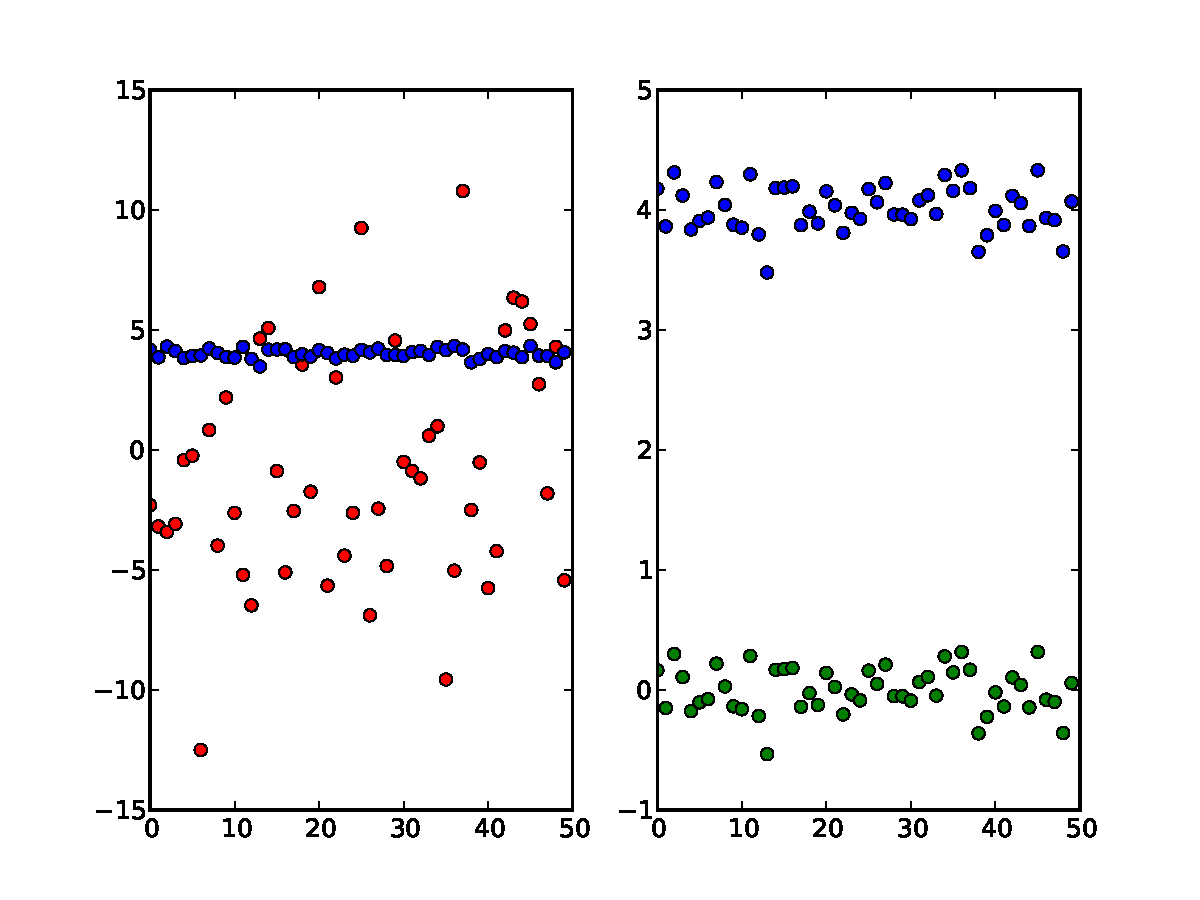
\includegraphics[width=\textwidth]{variance}
\caption{On the left, the red values come from a vector with relatively high variance,
         and the blue values come from a vector with relatively low variance.
         On the right, the green values have been shifted by the mean from the blue values.}
\label{fig:variance}
\end{figure}

Calculating the variance and the standard deviation in Python is straight forward.
Given the shifted data $X$, we simply square each entry, sum along the columns, and divide by the number of rows 
to obtain the variance. Take the square root of the result to get the standard deviation.
\begin{lstlisting}
>>> var = (X**2).sum(axis=0)/X.shape[0]
>>> var
array([ 260.     ,  193.42857,  176.28571,  151.14285])
>>> std = np.sqrt(var)
>>> std
array([ 16.124515,  13.907860,  13.277263,  12.294017])
\end{lstlisting}
Observe that the scores for the homework exhibited the largest amount of spread.

As with many things in Python, there is an even shorter, more convenient way to calculate these quantities. 
We may calculate the variance and standard deviation of the columns directly from $W$, without having to shift
by the mean.

\begin{lstlisting}
>>> var = W.var(axis = 0)
>>> var
array([ 260.     ,  193.42857,  176.28571,  151.14285])
>>> std = W.std(axis = 0)
>>> std
array([ 16.124515,  13.907860,  13.277263,  12.294017])
\end{lstlisting}

\begin{problem}
\label{prob:shiftdata}
Insert some problem here about importing some data, shifting by mean, finding row with the smallest variance, etc.
\end{problem}

\section*{The Inner Product and Angles Formula}

Inner products give information about lengths of vectors and angles between vectors. 
Recall that the standard inner product on $\mathbb{R}^n$ between vectors $x$ and $y$ is given by
$$
\ipt{x}{y} = x^T y = \displaystyle\sum_{i=1}^n x_iy_i.
$$
We can take advantage of convenient syntax in NumPy to quickly calculate the inner product between two vectors:
\begin{lstlisting}
>>> x = np.array([1., -2., 4.])
>>> y = np.arary([2., 3., -1.])
>>> (x * y).sum()
-8.0
\end{lstlisting}
The 2-norm of a vector can be easily recovered from the inner product:
\begin{lstlisting}
>>> x_norm = np.sqrt((x * x).sum())
>>> x_norm
4.5825756949558398
\end{lstlisting}
Another option to calculate the norm of an array is to use the \li{scipy.linalg.norm} function, which has the 
capability of computing a variety of different types of norms. For the purposes of this lab, however, our own
approach is perfectly sufficient (and even marginally faster).

Recall that the angle $\theta$ between two nonzero
vectors is given by
\[
\cos{\theta} = \frac{\ipt{x}{y}}{\norm{x}\norm{y}}
\]
where $\norm{x} = \sqrt{\ipt{x}{x}}$ denotes the 2-norm of $x$.
By bringing the constants into the inner product, we see that the angle satisfies
\[
\cos{\theta} = \left\langle\frac{x}{\norm{x}},\frac{y}{\norm{y}}\right\rangle.
\]
Hence, if we view the columns of $X$ as vectors in $\mathbb{R}^7$, we can find the cosine of the angles between these columns by dividing each
by its length, and then computing pairwise inner products. To divide the columns by their respective lengths, we may execute the following
code.
\begin{lstlisting}
>>> Y = X / np.sqrt((X**2).sum(axis = 0))
>>> Y
array([[ 0.39848615,  0.35329218,  0.11386819,  0.15371887],
       [-0.11720181, -0.16305793,  0.08540114, -0.12297509],
       [ 0.        , -0.02717632, -0.11386819,  0.        ],
       [-0.37504578, -0.48917378, -0.51240685, -0.27669396],
       [ 0.46880723,  0.54352643,  0.45547275,  0.49190037],
       [ 0.25784398,  0.27176321,  0.4839398 ,  0.43041282],
       [-0.63288976, -0.48917378, -0.51240685, -0.67636301]])
\end{lstlisting}

Finally, we get the cosines of the angles between columns by computing $Y^T Y$. To justify this calculation, consider
the $(i,j)^{th}$ entry of $Y^T Y$:
\begin{align*}
(Y^T Y)_{i,j} &= \sum_{k=1}^n (Y_{i,k})(Y^T)_{k,j} \\
&= \sum_{k=1}^n Y_{i,k}Y_{j,k} \\
&= \left\langle Y_{col i}, Y_{col j} \right\rangle,
\end{align*}
where $Y_{col i}$ denotes the $i^{th}$ column of $Y$, and $Y_{col j}$ the $j^{th}$ column.
Thus, we may obtain the cosine of the angle between each pair of columns of $X$ by computing $Y^T Y$,
which can be easily done in Python as follows:
\begin{lstlisting}
>>> np.dot(Y.T,Y)
array([[ 1.        ,  0.97782999,  0.89014869,  0.94908967],
       [ 0.97782999,  1.        ,  0.90978843,  0.92490144],
       [ 0.89014869,  0.90978843,  1.        ,  0.9276955 ],
       [ 0.94908967,  0.92490144,  0.9276955 ,  1.        ]])
\end{lstlisting}

We remark that the diagonals are always equal to one because the angle between a vector and itself is zero, and the cosine of zero is one.

%It is also worth noting that the matrix resulting from the operation $A \cdot A^T$ is symmetric and positive definite, so it compliant
%with the Cholesky decomposition that was discussed at the end of Lab \ref{lab:LUdecomp}.
% ^^ I'm not totally sure what is going on with this last statement. What exactly is A \cdot A^T? I'm assuming we mean A^T A, in which case
% the matrix is indeed only guaranteed to be positive semi-definite. It still has a Cholesky decomposition in theory, although I think it can only be
% computed for positive definite matrices. Anyway, I don't think the comment is relevant, so I have it removed for now.

\section*{Correlation}
In statistics, \emph{correlation} is a broad term that refers to various types of statistical relationships and dependence between 
variables of interest. 
In this setting, the \emph{Pearson correlation coefficient} of two vectors $u$ and $v$ is defined to be the cosine of the angle between the 
vectors $\overline{u}$ and $\overline{v}$, where $\overline{u}$ is the vector obtained by subtracting the mean of $u$ from each of its entries,
and similarly for $\overline{v}$. 
Two vectors are said to be
\begin{itemize}
\item Perfectly correlated if their correlation coefficient is one.
\item Positively correlated if their correlation coefficient is between zero and one.
\item Uncorrelated if their correlation coefficient is zero.
\item Negatively correlated if their correlation coefficient is between negative one and zero.
\item Perfectly anticorrelated if their correlation coefficient is negative one.
\end{itemize}

The notion of correlation is important in establishing linear relationships between measurements.  
Parallel vectors pointing in the same direction are perfectly correlated, since they lie in the same line.
Orthogonal vectors, on the other hand, are uncorrelated. 
Given two vectors of the same length, one can visually check for correlation by viewing a scatter plot.
This can be done in Python as follows:
\begin{lstlisting}
>>> from matplotlib import pyplot as plt
>>> x = np.random.rand(100)
>>> y = np.random.rand(100)
>>> plt.scatter(x,y)
>>> plt.show()
>>> plt.clf()
\end{lstlisting}
You will observe that the scatter plot does not indicate any obvious linear relationship between the two
vectors. You can calculate the correlation coefficient and confirm that it is close to zero.
See Figure \ref{fig:correlation} for examples of correlated and uncorrelated data.

\begin{figure}[h]
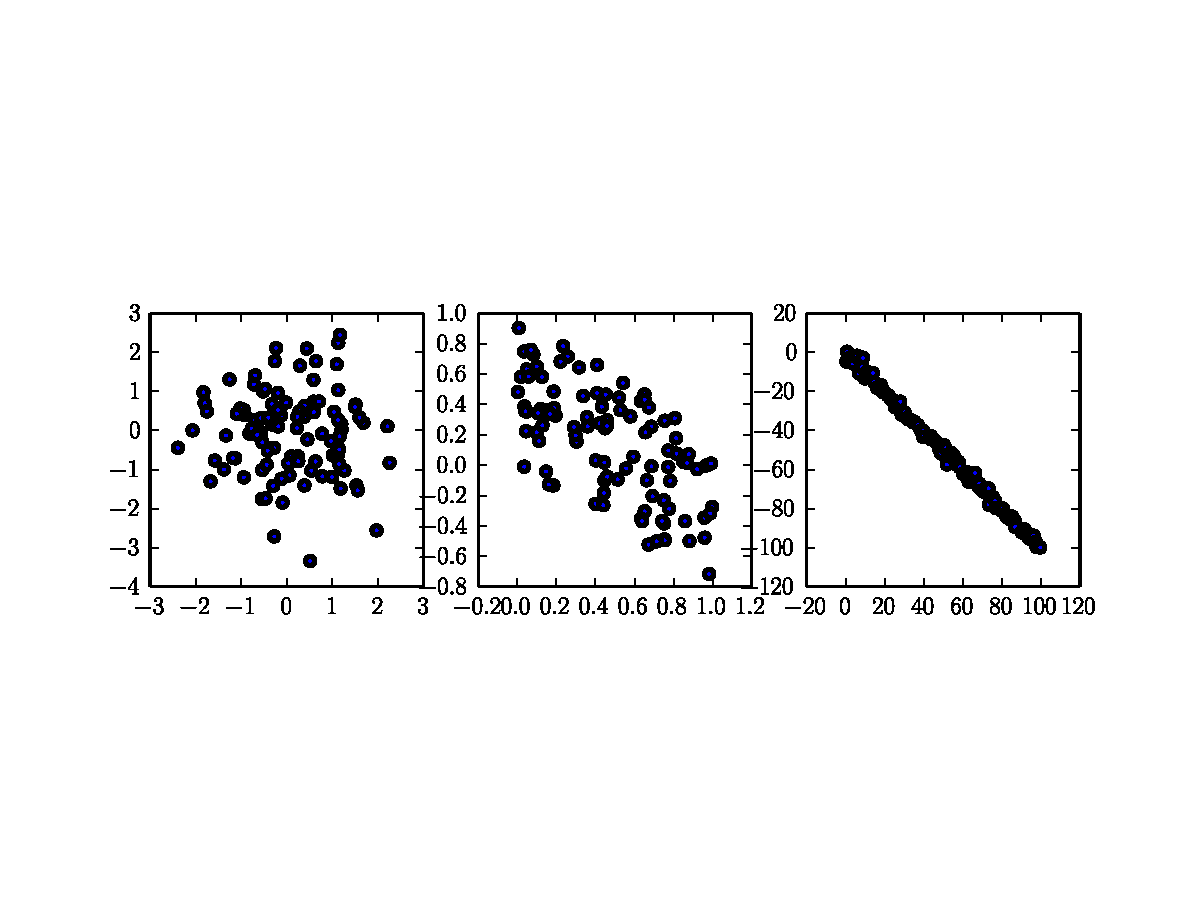
\includegraphics[width=\textwidth]{correlation}
\caption{Left: scatter plot of two slightly positively correlated vectors.
         Middle: scatter plot of two uncorrelated vectors.
         Right: scatter plot of two highly negatively correlated vectors.}
\label{fig:correlation}
\end{figure}
  
It's important to understand that the high correlation between quantities does not necessarily imply 
a causal relationship. For example, high correlation between violent crime rates and ice cream sales has 
been observed. This does not mean that ice cream causes crime or that increases in crime makes people want 
to eat more ice cream. Rather, both rates happen to increase during the summer and decrease during the winter.

Another import consideration is that the correlation coefficient does not provide information about 
non-linear relationships and dependencies between data. 

\begin{problem}
Load the data file \texttt{data.npy}.
The dataset consists of two columns.  Find the correlation coefficient of the two columns.  Then plot the original data and see if the value that you got is reasonable.
\end{problem}

The concepts of variance, standard deviation, correlation, and covariance apply to a much broader class of objects
known as \emph{random variables}, which are central to statistics and probability theory. These topics will be 
covered in detail later on. 
